\documentclass[titlepage,a4paper]{article}

\usepackage{a4wide}
\usepackage[colorlinks=true,linkcolor=black,urlcolor=blue,bookmarksopen=true]{hyperref}
\usepackage{bookmark}
\usepackage{fancyhdr}
\usepackage[spanish]{babel}
\usepackage[utf8]{inputenc}
\usepackage[T1]{fontenc}
\usepackage{graphicx}
\usepackage{float}

\pagestyle{fancy} % Encabezado y pie de página
\fancyhf{}
\fancyhead[L]{Apuntes Análisis de la información}
\fancyhead[R]{1C2021}
\renewcommand{\headrulewidth}{0.4pt}
\fancyfoot[C]{\thepage}
\renewcommand{\footrulewidth}{0.4pt}

\begin{document}
\begin{titlepage} % Carátula
	\hfill
\includegraphics[width=6cm]{logofiuba.jpg}
    \centering
    \vfill
    \Huge \textbf{Apuntes de análisis de la información}
    \vskip2cm
    \Large [7509] Análisis de la información\\
    Curso González \\
    1C 2021 
    \vfill
    \begin{tabular}{ | l | l | } % Datos del alumno
      \hline
      Alumno: & Grassano, Bruno \\ \hline
      Número de padrón: & 103855 \\ \hline
      Email: & bgrassano@fi.uba.ar \\ \hline
  	\end{tabular}
    \vfill
    \vfill
\end{titlepage}

\tableofcontents % Índice general

\newpage

\section{Introducción}\label{sec:intro}
El presente archivo contiene los apuntes que fueron tomados a lo largo de la cursada de la materia análisis de la información (7509) en el curso del profesor González.

% Grupos 5/6
% Final exposición de TP para coloquio. Evaluación de la exposición, calidad del trabajo, presentación, algunas preguntas teóricas individuales (solo sobre lo de los lunes)
% Nota final: Conceptual (Alejandro sobre el trabajo) + Exposición + Respuestas a preguntas teóricas


\section*{Primera clase}

    \begin{itemize}
        \item Introducción a la Ing. Software: Definiciones y metodología
        \item Modelos bajo el paradigma de OO
        \item Modelos de objetivos: Objetivo, alcance y hipótesis de un sistema
    \end{itemize}

\section{Introducción a la Ing. Software}
Definición: \textit{'Es la aplicación de un enfoque sistemático disciplinado y cuantificable al desarrollo, operación y mantenimiento de productos de software.'} (IEEE 1993) (Enfoque ingenieril)

\medskip

Otra definición: \textit{'Comprende principios y \textbf{metodologías} para desarrollar, operar y mantener software de calidad.'}


\subsection{Metodologías}
Contiene 3 partes. Los modelos, procesos, y las herramientas de un desarrollo de software. Estos son específicos a una metodología.

    \begin{itemize}
        \item Los modelos necesitan de un lenguaje de modelado $\rightarrow$ UML.
        \item Los procesos son \textit{XP, SCRUM, RUP, etc}
        \item Herramientas \textit{Suite Rational}
    \end{itemize}
    
    \begin{figure}[!htb]
        \centering
        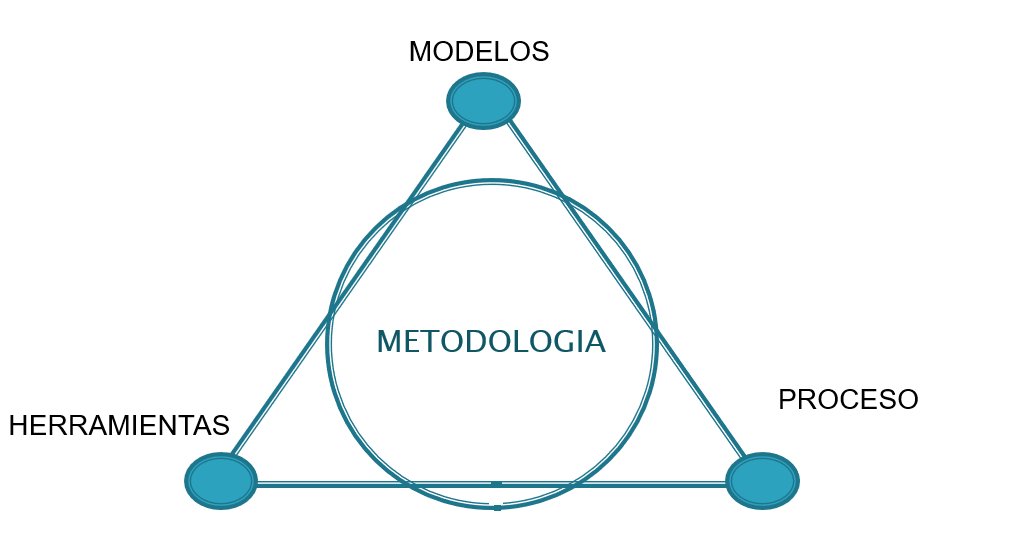
\includegraphics[width=0.8\textwidth]{Imagenes/Metodologias.png}
        \caption{Composición de una metodología}
    \end{figure}

\subsection{Modelos}
\subsubsection*{¿Que es un modelo?}
Es una simplificación de la realidad. Como la realidad es compleja le aplicamos abstracción, para incluir elementos que tienen mucha influencia y omitir los relevantes.

\subsubsection*{¿Para que sirve un modelo?}
    \begin{itemize}
        \item Para comprender mejor el sistema que estamos desarrollando.
        \item Para poder comunicarnos, con el cliente y el equipo de diseño.
        \item Visualizar y controlar rápidamente la arquitectura del sistema.
        \item Gestionar el riesgo de un proyecto. \textit{Calidad, plazos, y presupuesto}
    \end{itemize}

\subsubsection*{Etapas}
    \begin{itemize}
        \item Captura de requerimientos. \textit{Reuniones con cliente, cuestionarios, focus groups,...}
        \item Análisis de requerimientos: Es el ¿Que se necesita? \textit{Modelos de casos de uso, historias de usuario,...}
        \item Diseño: Es el ¿Como voy a hacer? \textit{Modelos de clases, de objetos, de despliegue,...}
        \item Construcción. \textit{Programación, integración de componentes...}
        \item Pruebas. \textit{Pruebas de sistema, unitarias, de usuario, de integración}
        \item Entrega. \textit{Despliegue del producto a los usuarios}
        \item Mantenimiento. \textit{Correctivo (Corregir defectos de diseño) y evolutivo (Adaptar a los nuevos procesos)}
    \end{itemize}

\subsubsection{Principios de la modelización}
    \begin{itemize}
        \item La elección de que modelos crear tiene una gran influencia sobre como se aborda un problema y como se da la solución.
        \item Tienen distintos niveles de precisión.
        \item Los mejores modelos tienen que estar ligados a la realidad.
        \item Un único modelo no es suficiente.
        \item Tener un Objetivo y alcance claro.
    \end{itemize}

\subsubsection{Beneficios de la modelización}
    \begin{itemize}
        \item Forma de visualizar necesidades y requerimientos contra costos reales antes de comenzar el desarrollo.
        \item Se trabaja en un alto nivel de abstracción
    \end{itemize}


\subsubsection*{Enfoques}
    \begin{itemize}
        \item Algorítmico
        \item Orientado a objetos
    \end{itemize}

\subsection{Paradigma orientado a objetos}
    \begin{itemize}
        \item Esta basado en la creación de componentes reutilizables.
        \item Construcción de software mas rápida y dinámica.
        \item Facilita la creación de prototipos.
    \end{itemize}

\subsection{UML}
Es un \textbf{lenguaje} estándar para escribir 'planos' de software. Lenguaje para visualizar, especificar, construir y documentar sistemas bajo el paradigma de orientación a objetos. Se utiliza desde el inicio hasta el fin del proyecto.
\textbf{No} es una \textbf{metodología}.

    \begin{figure}[!htb]
        \centering
        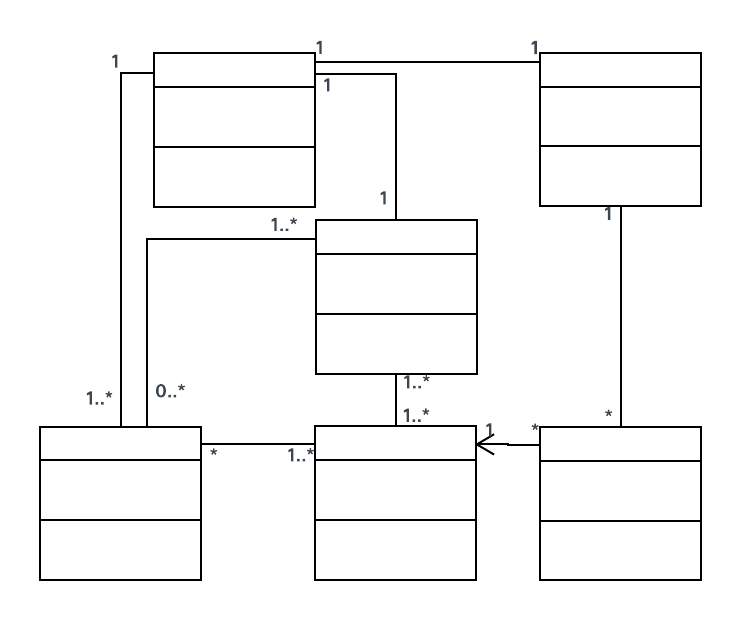
\includegraphics[width=0.5\textwidth]{Imagenes/UML.png}
    \end{figure}

\subsection*{Aspectos del modelado}
    \begin{itemize}
        \item Modelado funcional o de comportamiento. \textit{Historias de usuario}
        \item Modelado estático o estructural. \textit{Diagrama de clases}
        \item Modelado dinámico. \textit{Diagramas de interacción, secuencia}
    \end{itemize}

\subsection{Procesos de desarrollo de software}

Tiene que responder a 4 preguntas: ¿Quien lo hace?, ¿Que lo hace?, ¿Como lo hace?, ¿Cuando lo hace?
De forma tal de obtener un producto de calidad, dentro de plazos y presupuestos predecibles.

\section{Modelo de Objetivos}
\subsection{Objetivo del sistema}
Define lo que el sistema va a hacer (objetivo).
Es una descripción breve con alto nivel de abstracción, sobre \textbf{que} se requiere automatizar con el sistema, declarando los 'macroprocesos'.

\textit{Ej.
El sistema esta dirigido a administrar las ventas de la empresa, incluyendo la gestión de los pedidos del stock y la facturación de las mismas'.}

Macroprocesos involucrados: Gestión de pedidos, gestión de stock, gestión de facturación.

\subsection{Alcance del sistema}
Muestra los limites del objetivo(alcance). Para cada 'macroprocesos' hay que indicar las funcionalidades que el sistema va a contemplar,
dejando bien en claro que funcionalidades están \underline{dentro}/\underline{fuera} del alcance

Formato típico de un análisis del alcance.



\begin{table}[]
\begin{center}
\begin{tabular}{|l|l|c|}
\hline
\multicolumn{1}{|c|}{Macroproceso} & \multicolumn{1}{c|}{Funcionalidades} & Alcance \\ \hline
\textit{Nombre macroproceso}      & \textit{Nombre funcionalidad}       & \textit{Si/No} \\ \hline
 \multicolumn{1}{|c|}{...}          & \multicolumn{1}{c|}{...}            & ...            \\ \hline
\end{tabular}
\end{center}
\end{table}


\subsection{Hipótesis o supuestos funcionales}
Establece premisas o restricciones a tener en cuenta. (hipótesis)
Pueden ser establecidas por políticas de la empresa, normativas legales. Supuestos iniciales establecidos por el analista (deben ser verificados después por el cliente). No son requerimientos relevados, sino que complementan a los mismos.

Estos pueden darse por falta de relevamiento por determinadas circunstancias. \textit{Ej. El cliente se lo olvido, es trivial, no lo sabe, lo oculta}

\section{Caso de estudio: Airbus A320}

Habilitar la aceleración en reversa. El avión al momento de frenar activa este mecanismo, abriendo unos alerones en las turbinas.

El software: el piloto acciona el comando, ocurre un servo-mecanismo que abre los alerones. Caso de error a evitar, si el piloto lo acciona volando, tiene que haber algún mecanismo que detecte que el avión este en el piso. Se agrego un sensor de giro de ruedas, que detecta cuando giran en el piso y habilita la reversa del sistema que acciono el piloto.

El software salio de esta forma, pero tenia un problema, el avión estaba aterrizando, pero en caso de que la pista tenga hielo se producía un bloqueo y la rueda patinaba en vez de girar. Esto pasó debido a que no se contemplo en el universo en estudio.

Se debería de haber tenido en cuenta el sensor de giro, de peso, y de altura.

Sistema de estudio: software, los 3 sensores, el servo-mecanismo reversa.


\section*{Segunda clase}

    \begin{itemize}
        \item Modelo de negocio.
        \item Mapa de procesos.
        \item Mapa de sistemas.
        \item Diagrama de actividad.
    \end{itemize}

\section{Modelo de negocio}

\subsection{Mapa de procesos}
    \begin{itemize}
        \item Modeliza los procesos que una organización tiene para llevar adelante sus funciones.
        \item Permite entender la organización/negocio.
        \item Es un modelo matricial, modela los principales macroprocesos necesarios para el funcionamiento del negocio/empresa.
        \item Columnas: áreas del negocio. \textit{Ej. Estrategia y planificación, operación, previsión, assurance, billing}
        \item Filas: visión por capas. \textit{Ej. cliente, servicio, recurso, enterprise}
    \end{itemize}
    
    
    Conocer aquellos que vamos a automatizar, mas aquellos que interaccionan con el mismo.
    
\subsection{Mapa de sistemas}
    \begin{itemize}
        \item Modelo matricial: incluye los sistemas que dan soporte a los procesos de negocio.
        \item Columnas: áreas del negocio
        \item Filas: visión por capas
    \end{itemize}

Mapea determinados macroprocesos, y va diciendo cuales son los sistemas que van a automatizar los macroprocesos (mapa de sistemas) Puede ser mapeo 1 a 1, 1 a N, N a 1.

\subsection{Diagrama de actividad}
    \begin{itemize}
        \item Modeliza una secuencia de actividades en un escenario determinado. Modelo gráfico.
        \item Esta compuesto por un grafo dirigido. Los nodos son actividades, y los arcos (dirigidos) representan la transición entre actividades.
        \item Actividad de inicio, es única (circulo relleno) 
        \item Actividades de fin, puede haber varias (circulo con borde)
        \item El rombo (bifurcación) es de decisión. Indica caminos alternativos, elegidos según el valor de alguna expresión, surgida de un análisis que se lleva a cabo en una actividad.
        \item Barra de sincronización, agregar la barra indica que para que inicie otra actividad, tienen que haber finalizado todas las actividades que vayan a la barra.
        \item Dividiendo como columnas, agregar los responsables de cada actividad, quien las ejecuta. (Las 'Swimming lines', carriles, dividen las actividades')
        \item Estos diagramas no muestran temporalidad, esto esta en diagramas de secuencia.
        \item No muestran requisitos NO funcionales.
        \item Muy claro para comunicarse con el cliente y asegurarse de que se entendieron los requerimientos.
        \item Buen punto de partida para generar el modelo de comportamiento.
        \item Tipos de escenarios
        \begin{itemize}
            \item Global, contiene todos los procesos de negocio del universo en estudio.
            \item Parte del negocio, contiene algunos procesos de negocio del universo en estudio
            \item Un solo proceso de negocio, tiene todas las actividades de ese proceso.
            \item Regla de negocio, son las actividades de una regla de negocio.
        \end{itemize}
    \end{itemize}

    \begin{figure}[!htb]
        \centering
        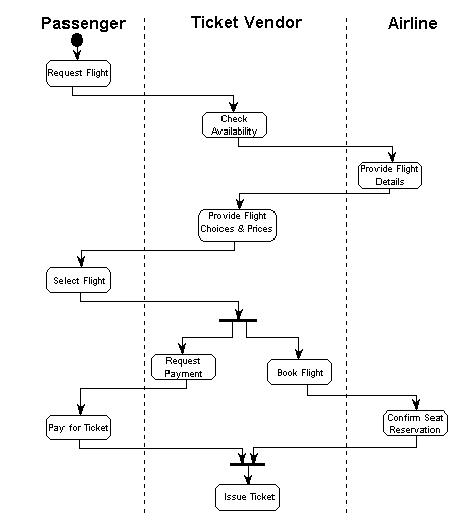
\includegraphics[width=0.7\textwidth]{Imagenes/DiagramaActividad.png}
        \caption{Diagrama de actividad. Notar las diferentes entidades: Actores, actividad de inicio (de fin falta), las secuencias, barras de sincronización.}
    \end{figure}

Una actividad esta compuesta por un conjunto de tareas a ser realizadas. Verbo $+$ objeto, \textit{ej. verificar pedido}. No hay que asociarlas con actividades físicas, si con procesos y/o reglas de negocio que luego podrán ser (o no) automatizadas.



\section*{Tercera clase}

\section{Modelo de comportamiento}
\subsection*{Casos de uso}

Hay tres componentes en el modelo de comportamiento.
\begin{itemize}
    \item Actores, representa algo o alguien (una persona, dispositivo, otro sistema) que interactúa con el sistema sin ser parte de el. Puede ingresar y/o recibir información del sistema. Se identifican fácilmente a partir de los roles representados por la swimline's. Se pueden identificar respondiendo a las siguientes preguntas: ¿Quien esta interesado en cierto requerimiento? ¿En que lugar de la organización se usa el sistema? ¿Quien se beneficiara con el uso del sistema? ¿Quien mantendrá el sistema? Etc.
    
    La clave para identificar buenos actores es pensar en el rol con el cual el actor interacciona con el sistema.

    \item Casos de uso, especifica el comportamiento de una parte del sistema. Representan un \textbf{requisito funcional} del sistema. Es un conjunto de acciones (variaciones incluidas) que ejecuta un sistema para producir un resultado para un actor. Gráficamente es una elipse con el nombre del caso de uso adentro.
    
    Son fácilmente identificables a partir del modelo de negocio (las actividades/tareas). Se pueden identificar con algunas preguntas también. ¿Cuales son las tareas de cada actor? ¿Que casos de uso crecerán, almacenaran, modificaran, consultaran, o eliminaran esta información? ¿Algún actor necesita informar al sistema sobre cambios externos? ¿Necesita algún actor ser informado de cambios en el sistema? Etc.
    
    Para identificar buenos y malos casos de uso, hay dos reglas.
    \begin{itemize}
        \item Completitud temporal, un caso de uso debe ser completo de principio a fin. \textit{Ej. Malos casos: seleccionar curso, registrar curso, informar registro (no son completos de principio a fin, cada uno esta en una parte, alumno, sistema)- Correcto: Registrar curso. (va del alumno al sistema)}
        \item completitud funcional, cuando varios casos de uso tratan con la misma entidad y son iniciados por el mismo actor podemos resumirlo en un solo caso de uso.\textit{Ej. Incorrecto: Departamento alumno: agregar curso, modificar curso, eliminar curso - Correcto: Mantener curso}
    \end{itemize}
    
    \item Diagramas de casos de uso, muestrea un conjunto de casos de uso, actores y sus relaciones. Permite tener una visualización del comportamiento de un sistema. En los diagramas de caso de uso general, se tiene una visión de alto nivel de todo el sistema, hay que tener 'todos' los actores y 'todos' los casos de uso del sistema. Hay actores primarios (izquierda diagrama)(disparan casos de uso) y actores secundarios (derecha diagrama)(no disparan casos de uso). Puede darse que un actor sea principal y secundario (esta en ambos lados).
\end{itemize}

%imagen actor (palito)


\subsection*{Documentación de casos de uso}
Tienen una descripción del caso, y flujo de eventos. (pre-condiciones, flujo principal, subflujos, flujos de excepción, post-condiciones)

Las pre-condiciones son las acciones que deben haber sido ejecutadas previas a la ejecución del caso de uso. 

Flujo de eventos, es una descripción de una secuencia de acciones necesarias para proveer la funcionalidad del sistema a un actor determinado.

Ej. Registrar curso a dictar.

\subsubsection*{Flujo principal}
\begin{enumerate}
    \item Profesor inicia en el sistema
    \item Sistema valida login (E1) y solicita ingresar cuatrimestre   [Las excepciones (flujo) se ponen entre paréntesis]
    \item Profesor ingresa cuatrimestre
    \item Sistema solicita ingresar acción a ejecutar - Agregar, Modificar, Eliminar, Salir
    \item Profesor ingresa acción
    [Comienzan los subflujos]
    \begin{itemize}
        \item Agregar: Ejecutar subflujo S1: Agregar Curso a dictar
        \item Modificar: Ejecutar sublfujo S2: Modificar curso a dictar
        ...
    \end{itemize}
\end{enumerate}

\subsubsection*{Subflujo S1 Agregar Curso a dictar}
\begin{enumerate}
    \item Sistema solicita ingresar materia
    \item profesor ingresa materia (E2)
    \item Sistema muestra los cursos correspondientes a la materia
    \item Profesos selecciona los cursos a dictar
    \item Sistema registra al profesor en los cursos seleccionados
    \item El caso de uso comienza nuevamente en Sistema solicita ingresar acción a ejecutar    [Se indica donde se sigue]
\end{enumerate}

\subsubsection*{Excepción E1}
\begin{enumerate}
    \item Sistema solicita reingresar login o finalizar caso de uso.
    \begin{enumerate}
        \item Ingresa login y continua en 2.
        \item Finaliza casos de uso.
    \end{enumerate}
\end{enumerate}


\subsection*{Tipos de relaciones}
\begin{itemize}
    \item De asociación entre actores y casos de uso.
    \item De dependencia entre casos de uso. 2 tipos, de inclusión <<INCLUDE>> y de extensión <<EXTEND>>
    
    <<INCLUDE>> es para evitar repetir en varios casos de uso el mismo flujo de eventos. Llevo los casos comunes a un nuevo caso de uso común a ambos. Gráficamente es una linea punteada con <<INCUDE>>. La llamada del flujo de eventos es ... \\n Include(Validar Usuario)  \\n ...
    
    <<EXTEND>> se usa cuando en un caso de uso determinados eventos se dan solamente bajo ciertas condiciones. Gráficamente la flecha es punteada y va desde el caso de uso extendido al caso de uso base. El caso de uso base no se entera si se ejecuta el caso de uso extendido. Va acompañado por una etiqueta que tiene que coincidir en el flujo.
    
    \item De generalización/especialización entre actores/entre casos de uso.
\end{itemize}

%imagen <<include>>

\section*{Cuarta clase}
\subsection*{Caso de uso: Actor temporal}
Indica el paso del tiempo, tiene una flecha punteada hacia el caso de uso. %agregar imagen

\subsection*{Caso de uso: Relaciones de especialización/generalización}
Son actores que pueden tener una flecha hacia otro actor, para indicar que puede iniciar los casos de uso de ese otro actor.

\section{Proceso de desarrollo iterativo e incremental}
Voy realizando pequeñas partes del proyecto total. En cada iteración se van capturando requerimientos, análisis, diseño, construcción, testeo y despliegue. Es un mini ciclo de cascada. Cada iteración dura entre 2 y 6 semanas, esto permite que el usuario este probando mucho antes en comparación a cascada (interacción con el usuario constante). Ante cualquier error que ocurra, se esta a tiempo de arreglarlo.

\section{Casos de Uso 2.0}
Un slice es una porción de un caso de uso. Estos son hechos durante cada iteración del desarrollo iterativo e incremental.
% todo: completar...

Busca partir los casos de uso en porciones mas pequeñas, para que sean mas implementables en el lapso de 2 a 6 semanas. Proporciona mucha versatilidad.

\section{Historias de usuario}
Las historias de usuario son descripciones breves y simples de una funcionalidad, escritas desde la perspectiva que necesita una determinada capacidad del sistema. \textit{Ej. Usuario, área de negocio, o cliente}

\subsection*{Componentes}
\begin{itemize}
    \item ID
    \item Titulo: Texto descriptivo de la historia
    \item Descripción: Como [rol], quiero [objetivo], para poder [beneficio]
    \item Estimación: Cuanto va a llevar implementarla (conocida también como puntos de historia)
    \item Valor: valor numérico que aporta importancia a la historia, generalmente de 1 a 5. El objetivo es maximizar el valor y la satisfacción percibida por el cliente o usuario en cada iteración.
    \item Dependencias: Procurar que no existe dependencia entre historias, los que no sea posible indicarla.
    \item Pruebas de integración: Clarifican el contexto en que ocurre la historia, y facilitan saber cuando están terminadas las historias.
\end{itemize}

Ej. 
\begin{itemize}
    \item COMO usuario QUIERO poder acceder al catalogo de cursos PARA poder tomar decisiones de los cursos en los cuales inscribirme.
    \item COMO usuario QUIERO poder buscar transacciones PARA poder detectar gastos innecesarios en mi cuenta durante cierto periodo de tiempo.
\end{itemize}

\subsection*{Buenas practicas}
\begin{itemize}
    \item Deben mapear a \textbf{una sola} funcionalidad del producto, software.
    \item Es una buena practica usar personajes en vez de roles. \textit{Ej. Alumno en vez de usuario}.
    \item Se hacen en fichas.
\end{itemize}

\subsubsection*{INVEST}
\begin{itemize}
    \item Independiente: No deben depender unas de otras, si ocurre tratar de dividir o combinar.
    \item Negociable: Deben ser negociables sus detalles entre cliente/usuario en la <<conversación>>.
    \item Valor: Tiene que ser valiosa para el cliente.
    \item Estimable: Debe ser estimada con la precisión suficiente para ayudar al cliente o usuario a priorizar y planificar su implementación.
    \item Pequeña (Small): Como máximo una iteración.
    \item Testeable: Deben poder probarse y saber que la historia se completo con éxito.
\end{itemize}

\subsection*{Criterios de aceptación}
Son una serie de preceptos que validan la implementación de la historia de usuario.
\begin{itemize}
    \item Ayudan al desarrollador a implementarla de forma correcta.
    \item Se pueden mapear sobre los tests de funcionalidades.
    \item Ayudan a QA para dar el OK a la historia.
    \item Definen junto a la descripción la funcionalidad a implementar.
    \item Tienen solo 2 resultados: ÉXITO o FRACASO.
    \item Deben ser interpretados de una única manera por N personas, no deben ser ambiguos.
    \item Deben ser verificables por el cliente rápidamente.
    \item Tienen que ser completos, el grupo debe incluir todas las funcionalidades.
\end{itemize}

Ej.
\begin{itemize}
    \item El nombre de usuario DEBE tener un valor, en caso contrario se mostrara el mensaje de error pertinente.
    \item Si el usuario y la contraseña son correctos, el usuario podrá acceder a la aplicación.
\end{itemize}

\subsection*{Conversaciones}
En el mundo ideal los clientes tienen una idea muy clara de lo que quieren desde el principio, y nos lo cuentan con lujo de detalles sin dejarlo en el tintero. En la realidad esto no pasa.

Una historia de usuario abrirá normalmente una conversación entre el equipo de desarrollo y el cliente. Las historias de usuario no cambian a nivel conceptual, son las conversaciones las que las volverán mas detalladas.


\section*{Quinta clase}

\section{Modelo Conceptual}
Dentro de los modelos de requerimientos.

\subsection{Diagramas de clases conceptuales}
Las clases representan los bloques de construcción mas importantes de cualquier sistema.

\begin{itemize}
    \item Nombre
    \item Atributos: propiedades del elemento que estamos modelando
    \item Operaciones (Métodos): implementación de un servicio
    \item Responsabilidades: lo que le corresponde realizar a la clase,las obligaciones que deben realizar las clases para cumplir con los requerimientos. \textit{Ej. determinar el riesgo de un pedido de un cliente - manejar criterios de fraude específicos del cliente}
\end{itemize}

% imagen de clase

Es buena practica iniciar el modelaje especificando las responsabilidades, dejando para después los atributos y operaciones. Deben de contener al menos 'una' responsabilidad. (tratar de respetar el Single Responsability Principle)

Las clases conceptuales (de entidad), son las necesarias para cumplir con las responsabilidades asignadas al sistema.

Clase de entorno, maneja el dialogo entre el sistema y el medio externo.

Para identificar clases, se puede usar la regla practica, usar sustantivos o frases sustantivas que describen responsabilidades del sistema. La otra forma es con tarjetas CRC (Colaboration Responsability Card), que es una técnica de modelado para refinamiento de clases.

De aca se tiene una lista inicial de clases, y con esto se hace un diagrama de clases participantes (sin colaboraciones).

\subsubsection*{Relaciones entre clases}
\begin{itemize}
    \item De asociación, es entre instancias que se encuentran en un mismo nivel. Tiene nombre de asociación, rol, multiplicidad. Existen la simple, de agregación, de composición y clase de asociación
    
    \begin{itemize}
        \item Simple, relación de asociación entre objetos de una clase. \textit{Ej, Nombre de asociación: Emplea} Recta que une las dos clases. El rol puede omitirse si es trivial. La multiplicidad es obligatoria.
        \item Agregación, se tiene una clase que representa un todo, y otra una parte. Si se elimina una instancia del todo, las partes siguen existiendo. Tiene un rombo vacío del lado del todo.
        \item Composición, fuerte relación de pertenencia y vida entre un todo y las partes. Si se elimina e todo, las partes asociadas mueren. Rombo negro del lado del todo. Un todo puede tener muchas partes, pero no puede haber una parte de muchos todos.
        \item Clase de asociación, es una nueva clase que surge de la asociación de dos clases, contiene elementos que no le son propios a las clases relacionadas. Existen una sola vez, si se repite se convierte asociación simple.
    \end{itemize}
    
    \item De generalización, especialización: Es una relación que conecta una clase general con una mas especializada. (Subclase) La clase hijo siempre es instanciable, la padre puede o no serlo. Si no lo es, se dice abstracta. el discriminador indica en base a que especializo.
    
    \item De uso, dependencia,
    \item De realización, interfaces
\end{itemize}


\section*{Sexta clase}
\section{Diagramas de interacción entre objetos}
La interacción entre objetos comprende el conjunto de mensajes que son intercambiados entre objetos.

Estos diagramas describen la manera en que colaboran grupos de objetos para cierto comportamiento. Se usan cuando se quiere ver el comportamiento en un escenario predefinido.

Ambos tipos de diagramas son equivalentes. De cada uno puedo llegar al otro. Se enumeran los mensajes en ambos.

\subsection{Diagrama de secuencia}
Muestran el orden temporal de los mensajes y el paso de mensajes. 'Perspectiva cronológica de las interacciones'.

% diagrama

\subsection{Diagrama de colaboración}
Muestra la organización estructural de los objetos que envían y reciben mensajes. 'Perspectiva espacial de las interacciones'

Linea entre objetos que intercambian mensajes y otra linea indicando la dirección.

% diagrama



\newpage

\section{Bibliografía de la materia}

\begin{itemize}
    \item The Unified Modeling Language Reference Manual, Rumbauch, Jacobson, Booch
    \item The Unified Software Development Process, Rumbauch, Jacobson, Booch
    \item UML distilled, Third Edition, Fowler
\end{itemize}

\end{document}
